\documentclass[10pt,letterpaper]{article}
\usepackage[top=0.75in, left=0.5in, right=0.5in, footskip=0.5in]{geometry}

% Include FloatBarrier  
\usepackage{placeins}
% Use adjustwidth environment to exceed column width (see example table in text)
\usepackage{changepage}
% Use Unicode characters when possible
\usepackage[utf8]{inputenc}
% textcomp package and marvosym package for additional characters
\usepackage{textcomp,marvosym}
% fixltx2e package for \textsubscript
\usepackage{fixltx2e}
% amsmath and amssymb packages, useful for mathematical formulas and symbols
\usepackage{amsmath,amssymb}
% cite package, to clean up citations in the main text. Do not remove.
\usepackage{cite}
% Use nameref to cite supporting information files (see Supporting Information section for more info)
\usepackage{nameref,hyperref}
% line numbers
\usepackage[right]{lineno}
% ligatures disabled
\usepackage{microtype}
\DisableLigatures[f]{encoding = *, family = * }
% rotating package for sideways tables
\usepackage{rotating}
% Remove comment for double spacing
%\usepackage{setspace} 
%\doublespacing

% Text layout
\raggedright
\setlength{\parindent}{0.5cm}
\textwidth 5.25in 
\textheight 8.75in

% Bold the 'Figure #' in the caption and separate it from the title/caption with a period
% Captions will be left justified
\usepackage[aboveskip=1pt,labelfont=bf,labelsep=period,justification=raggedright,singlelinecheck=off]{caption}

% Use the PLoS provided BiBTeX style
\bibliographystyle{plos2015}

% Remove brackets from numbering in List of References
\makeatletter
\renewcommand{\@biblabel}[1]{\quad#1.}
\makeatother

% Leave date blank
\date{}

% Header and Footer with logo
\usepackage{lastpage,fancyhdr,graphicx}
\usepackage{epstopdf}
\pagestyle{myheadings}
\pagestyle{fancy}

%% Include all macros below

\newcommand{\lorem}{{\bf LOREM}}
\newcommand{\ipsum}{{\bf IPSUM}}

%% END MACROS SECTION


\begin{document}
\vspace*{0.35in}

% Title must be 250 characters or less.
% Please capitalize all terms in the title except conjunctions, prepositions, and articles.
\begin{flushleft}
{\Large
\textbf\newline{Volume Gradient Vector}
}
\newline
% Insert author names, affiliations and corresponding author email (do not include titles, positions, or degrees).
\\
%Name1 Surname\textsuperscript{1,\Yinyang},
%Name2 Surname\textsuperscript{2,\Yinyang},
%Name3 Surname\textsuperscript{2,\textcurrency a},
%Name4 Surname\textsuperscript{2,\ddag},
%Name5 Surname\textsuperscript{2,\ddag},
%Name6 Surname\textsuperscript{2},
%Name7 Surname\textsuperscript{3,*},

%\\
%\bigskip
%\bf{1} Affiliation Dept/Program/Center, Institution Name, City, State, Country
%\\
%\bigskip

* CorrespondingAuthor@institute.edu
\end{flushleft}

%%%%%%%%%%%%%%%%%%%%
%%%%%% ARTICLE %%%%%
%%%%%%%%%%%%%%%%%%%%
\linenumbers
\section{Abstract}
asd
\newpage
\section{Introduction}
asd



\newpage
\section{Methods}

Essential modes (EMs) were extracted from 600ns production run and normalized to a length of 6 \AA . Then, the average structure was displaced along each EM and the derivatives of the volumes (\(\delta V_{i}\)) calculated. Since higher order EMs tend to be localized in a few amino acids, applying the same magnitude of displacement along each EM coud lead to excessive displacements, causing atom clashes. Thus, each displacement vector \(\mathbf{D}_i\) was scaled by the following formula:
$$
\mathbf{D}_i = \frac{1}{l_i} \cdot \mathbf{Q}_i
$$
were \(l_i\) is the frequency of the corresponding essential mode.
The (\(\delta V_{i}\)) were compiled in a  \textbf{Volume Gradient Vector} (\textbf{VGV}) which then was used to select the subset of modes that affect the cavity the most by means of the \textbf{Participation Number} (\(\mathbf{P}\)):
$$
P = ({\sum_i {(\mathbf{VGV} \cdot \mathbf{Q}_i)}^4})^{-1}
$$
the \({P}\) is rounded and used to determine the size of the subspace. The '\({P}\)' modes that have the higher projections against the \textbf{VGV} are selected.\newline

The \textbf{VGV} may be transformed to cartesian coordinates to determine wich amino acids affect the cavity the most. Each EM can then be cutted to keep the displacements of the wall amino acids, discarding the rest of the vector. This cutting procedure was applied to the 2 sets of EMs: the whole subspace, and the '\({P}\)' modes. \textbf{Collectivity} and \textbf{Participation Number} of each mode were recalculated to these cutted set of modes.\newline

The \textbf{collectivity} of each mode was calculated using the formula from Tama et.al.:
$$
formula
$$\newline

The \textbf{Participation Number} formula was also used to determine the number of amino acids that each EM mainly moves. These '\({P}\)' amino acids of each mode was divided by the total numbre of amino acids to obtaint the fraction of the protein that is affect the most by each mode.




\newpage
\section{Results}
\subsection{1HVR\_APO}
Fig.1 shows density of states histograms of the EM, weighted by the (\(\delta V_{i}\)) of each mode. Fig.1A corresponds to the full set of EM and Fig.1B for the reduced set of 149 '\(P\)' modes. These plots can be compared with a non-weighted density of states histogram (Fig.1C). (\textbf{se me ocurre q podríamos ponerlo acá}) Despite being the most numerous, middle frequency modes (\({50cm}^{-1}\) to \({175cm}^{-1}\)) are not so relevant to the cavity volume and low frequency modes turn out to be even more important. Notably, a spike appears between the range of    \({175cm}^{-1}\) to \({200cm}^{-1}\); these modes could indicate an alternative way of affecting the cavity volume. Besides a 'breathing' movement, encapsulated in the lower frequency amino acids, a protein could use the coordinated movement of several amino acids to affect the cavity volume or to function as a gate. If these residues undergo coordinated movement, then the gating dynamics should show up in middle frequency EM.
\clearpage

\begin{figure}[ht]
\begin{center}
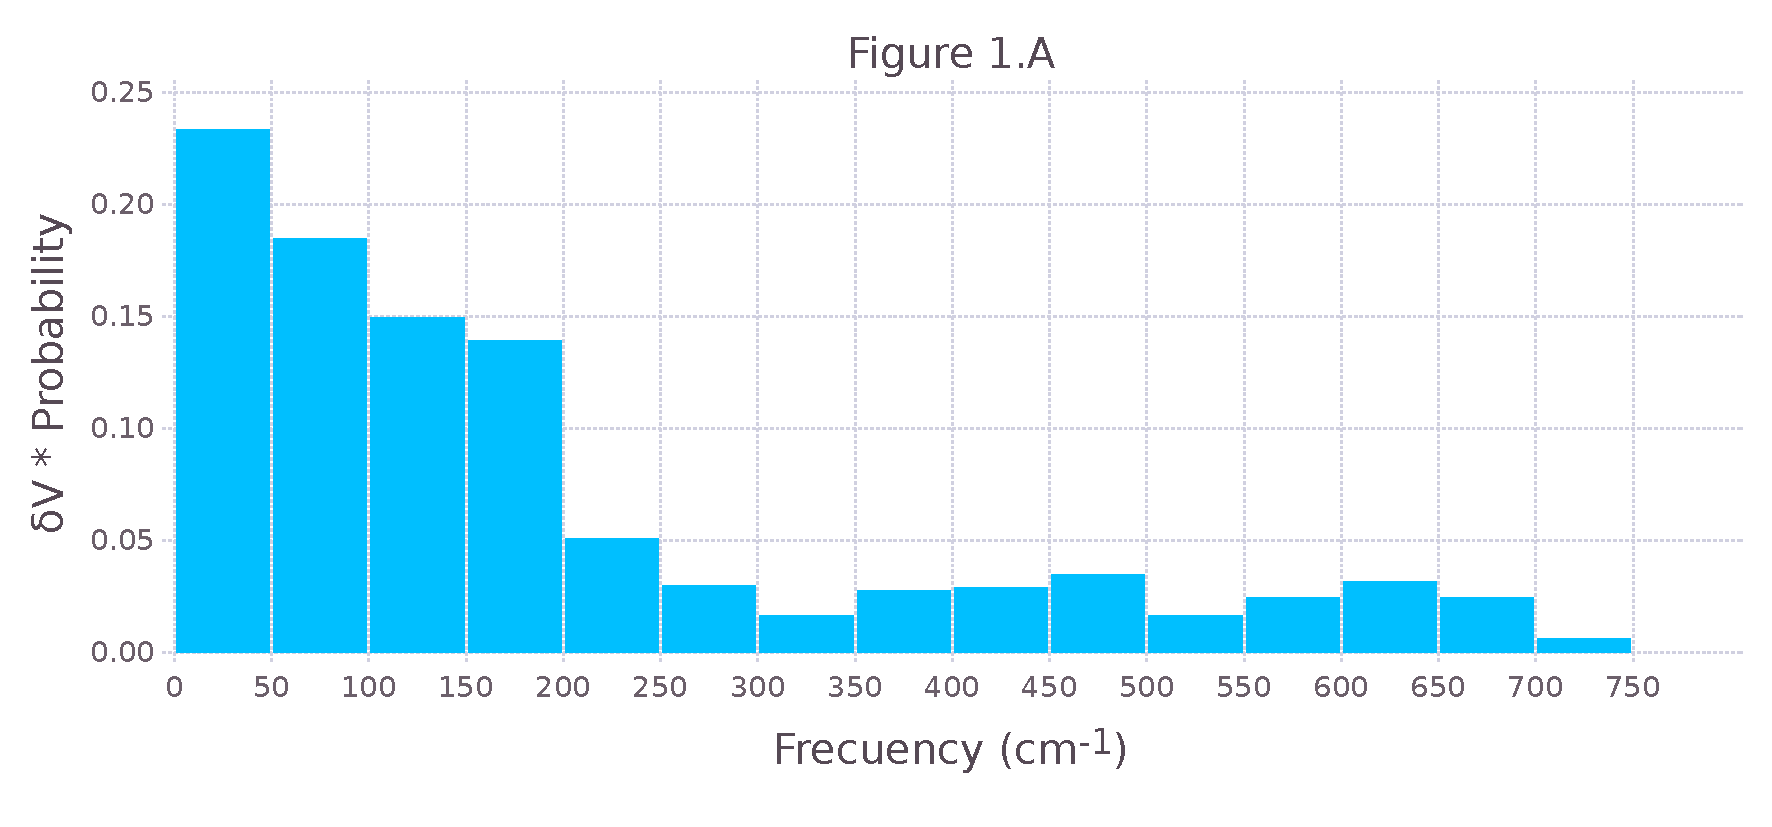
\includegraphics[scale=0.5]{1hvr_apo/1afigure.pdf}
\caption{This is an inserted EPS graphic}
\label{fig1}
\end{center}
\end{figure}

\begin{figure}[ht]
\begin{center}
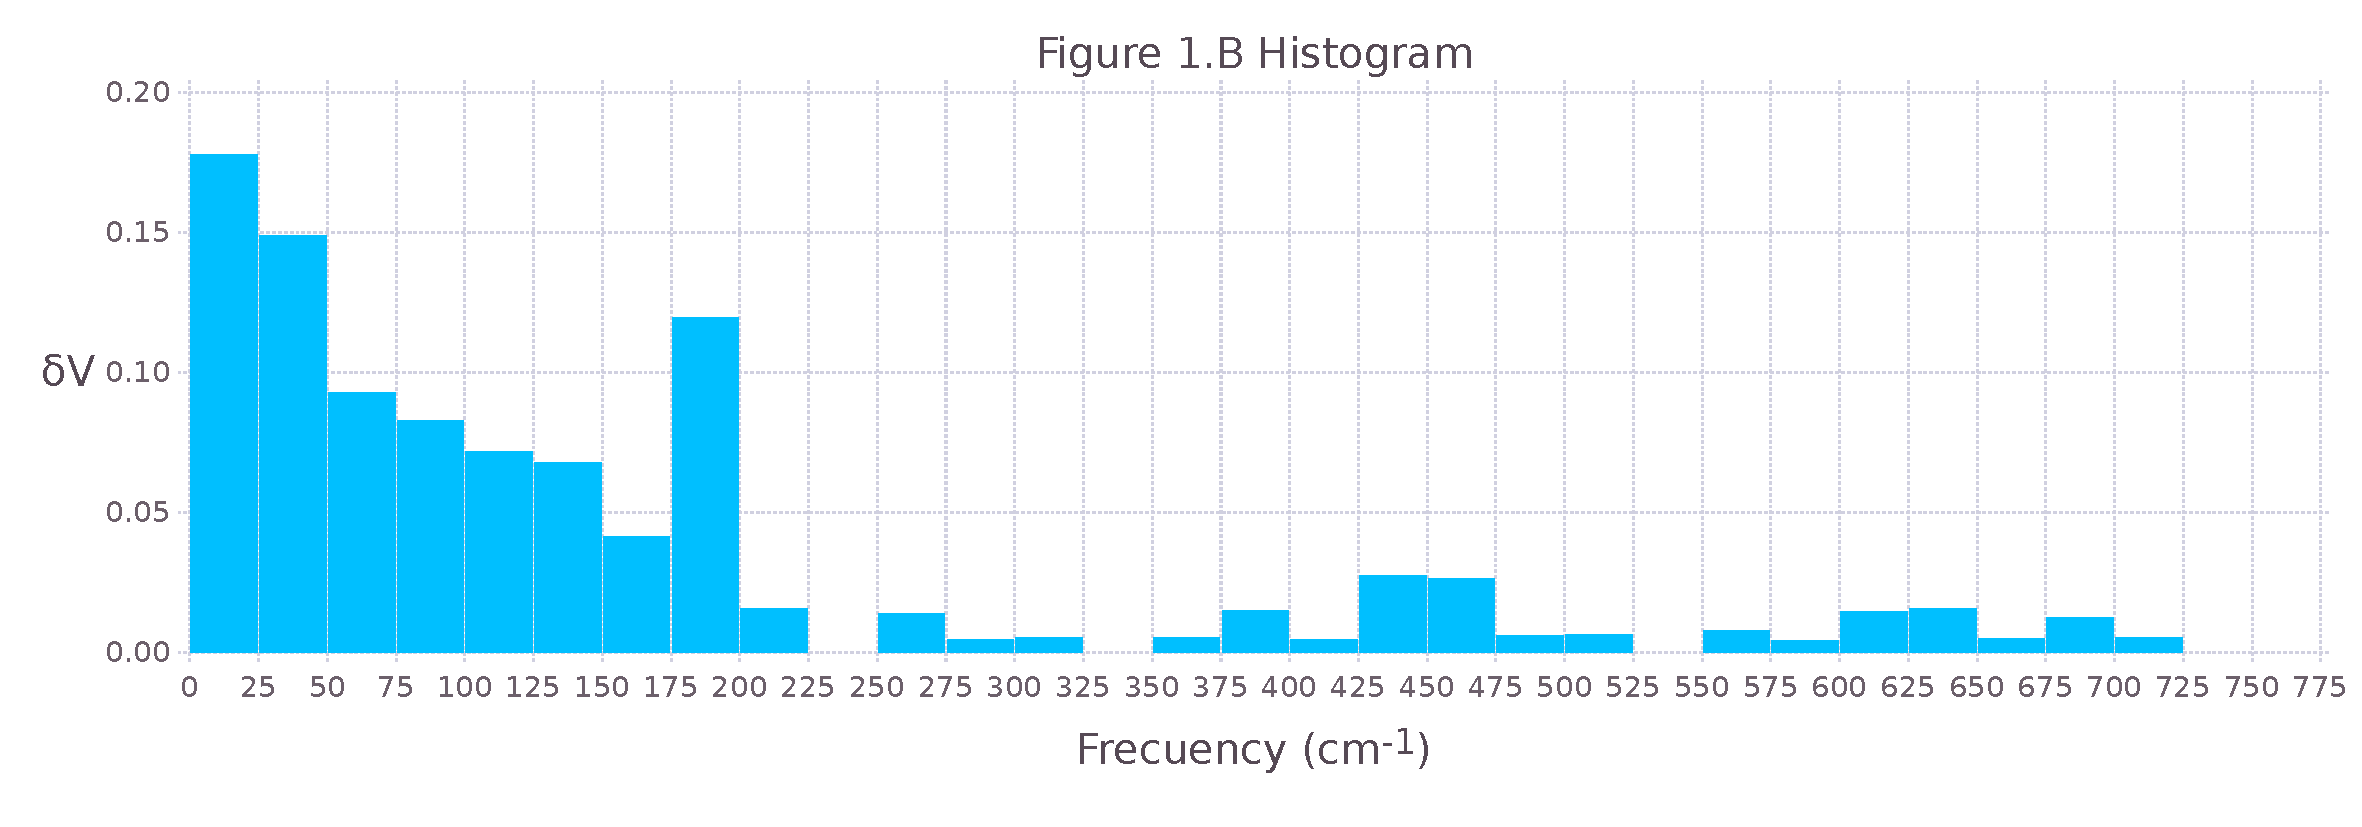
\includegraphics[scale=0.5]{1hvr_apo/1bfigure.pdf}
\caption{This is an inserted EPS graphic}
\label{fig2}
\end{center}
\end{figure}

\clearpage
As in Fig.1, the analogous can be done with collectivity, as Fig.2 shows. 

\begin{figure}[ht]
\begin{center}
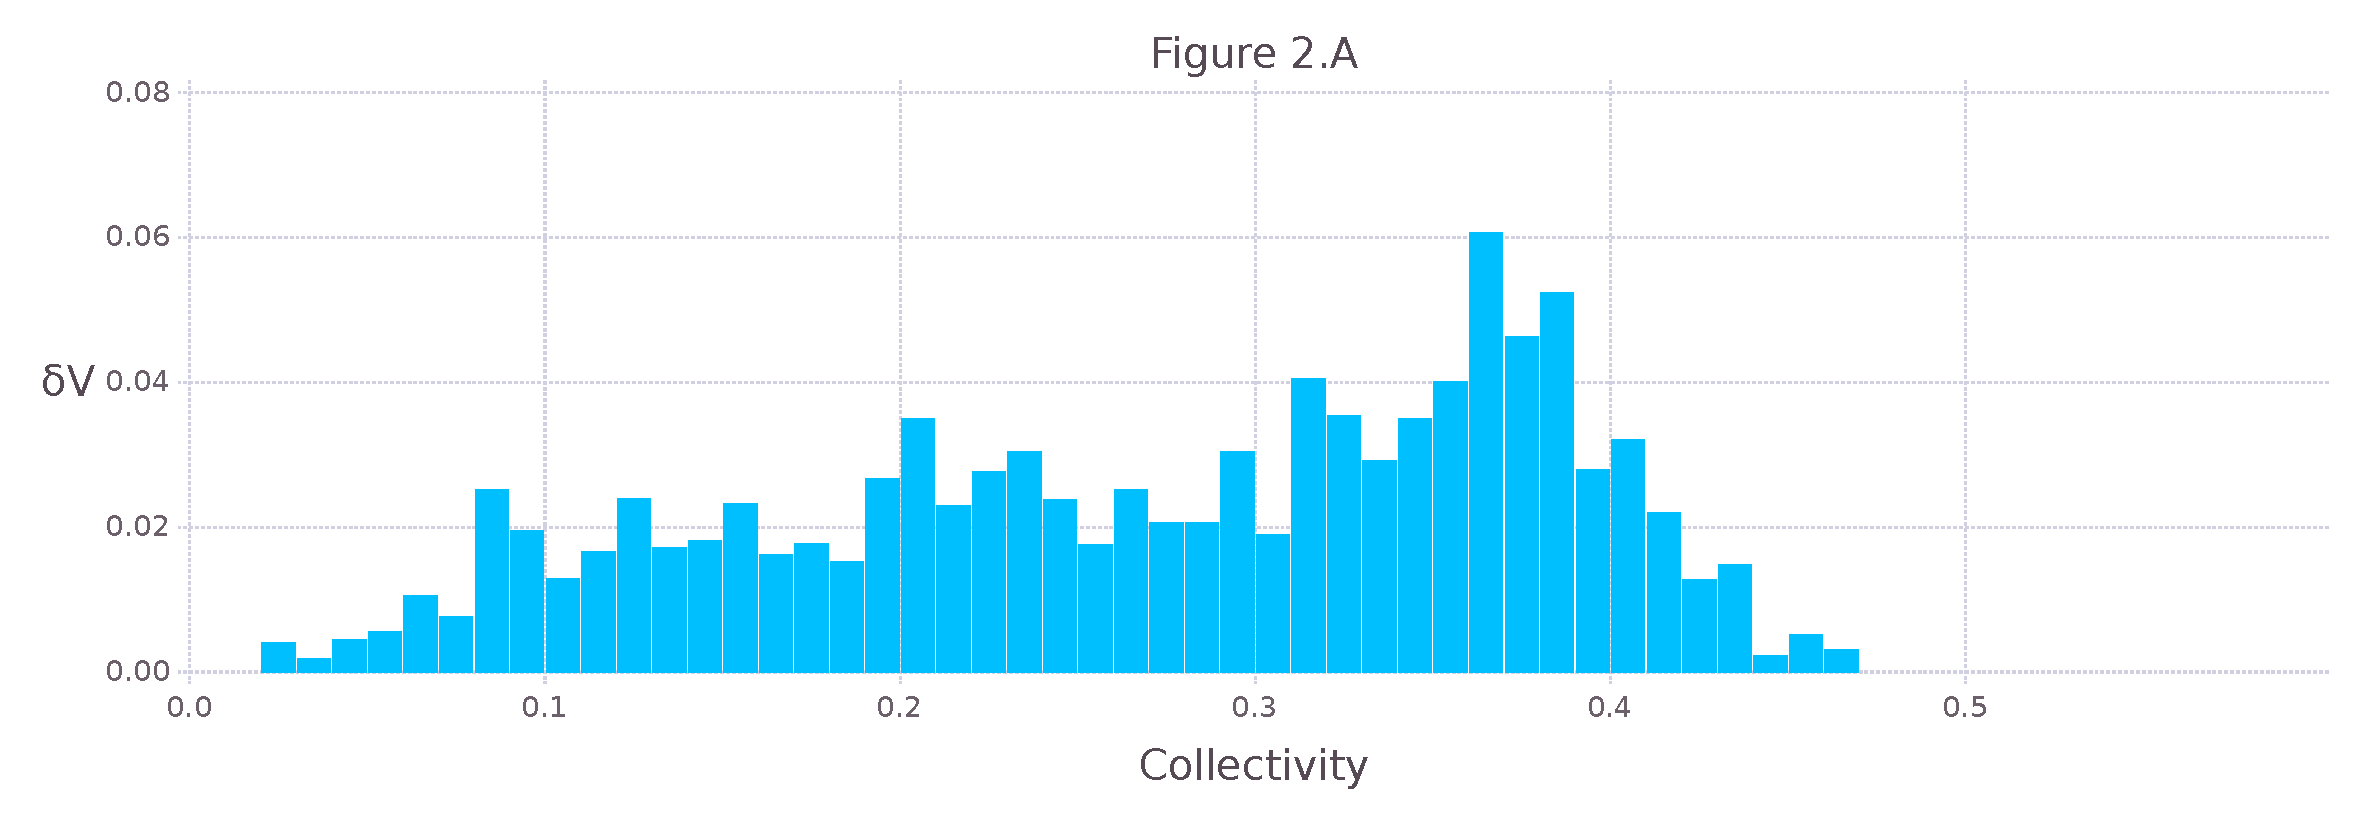
\includegraphics[scale=0.5]{1hvr_apo/2afigure.pdf}
\caption{This is an inserted EPS graphic}
\label{fig3}
\end{center}
\end{figure}

\begin{figure}[ht]
\begin{center}
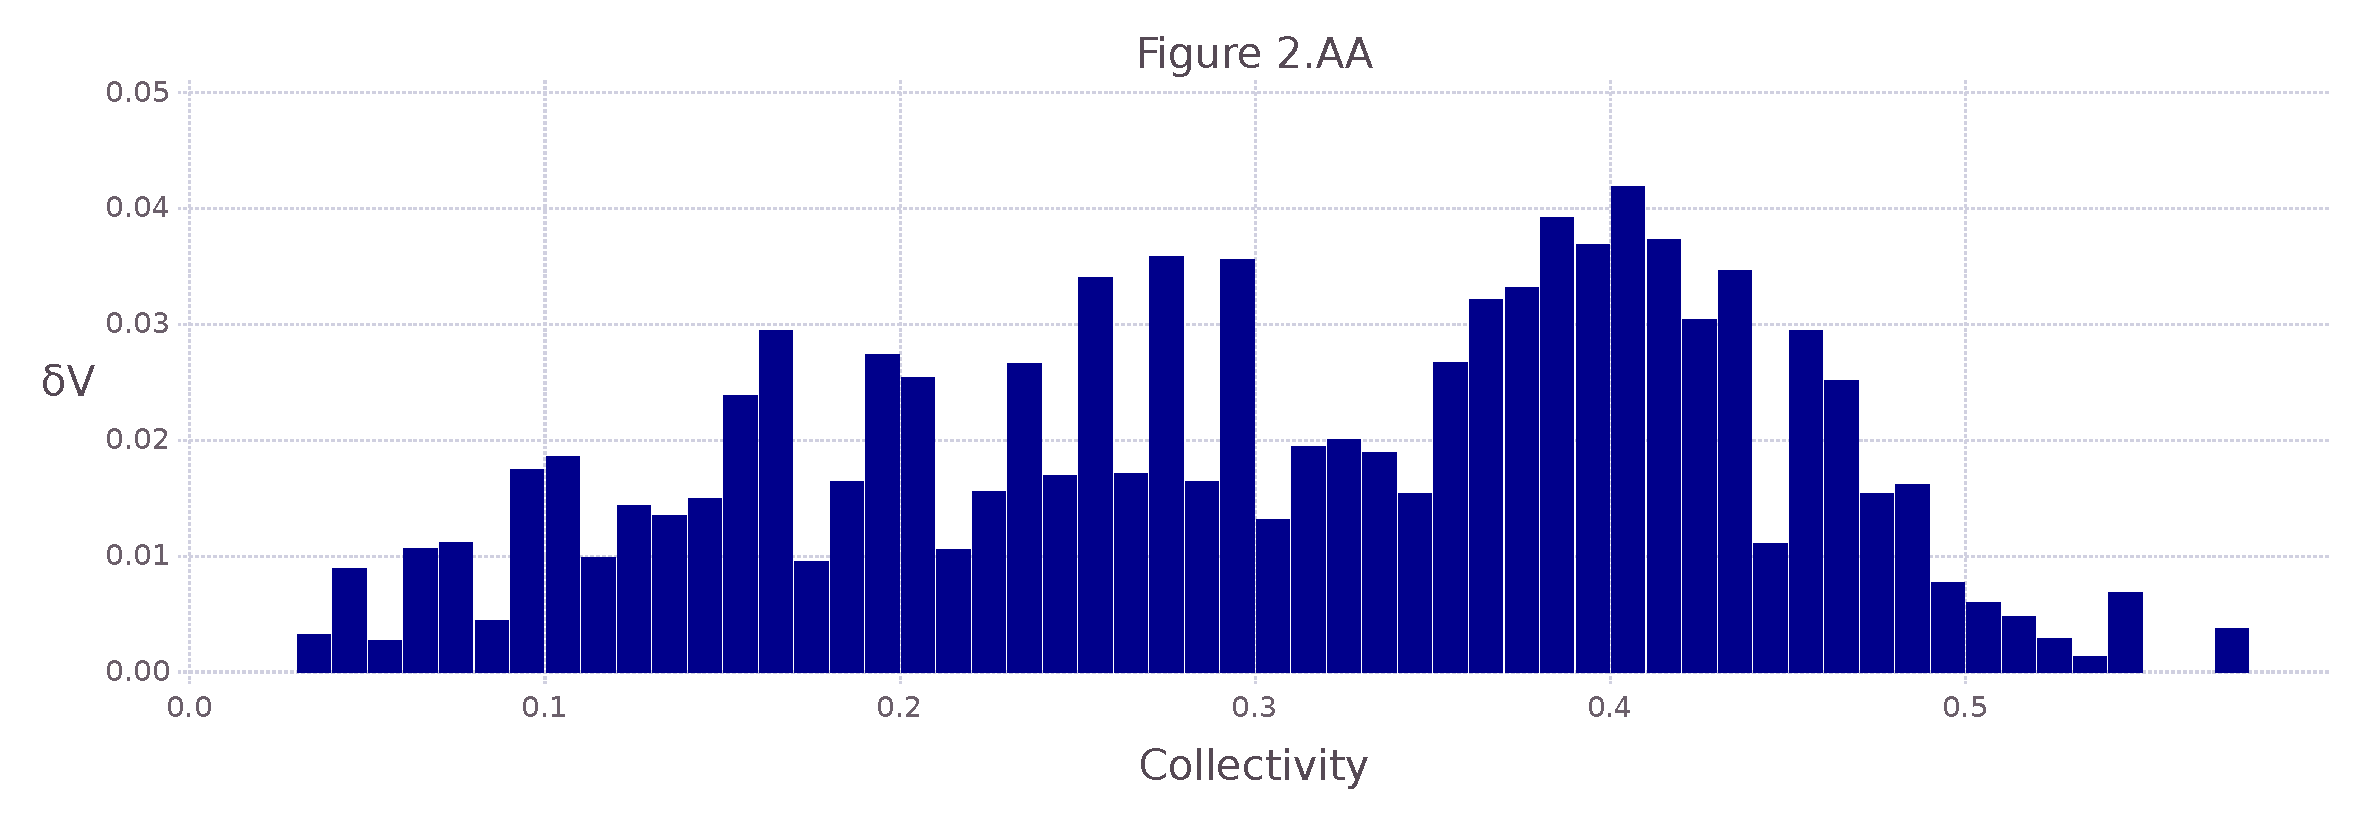
\includegraphics[scale=0.5]{1hvr_apo/2aafigure.pdf}
\caption{This is an inserted EPS graphic}
\label{fig4}
\end{center}
\end{figure}

\begin{figure}[ht]
\begin{center}
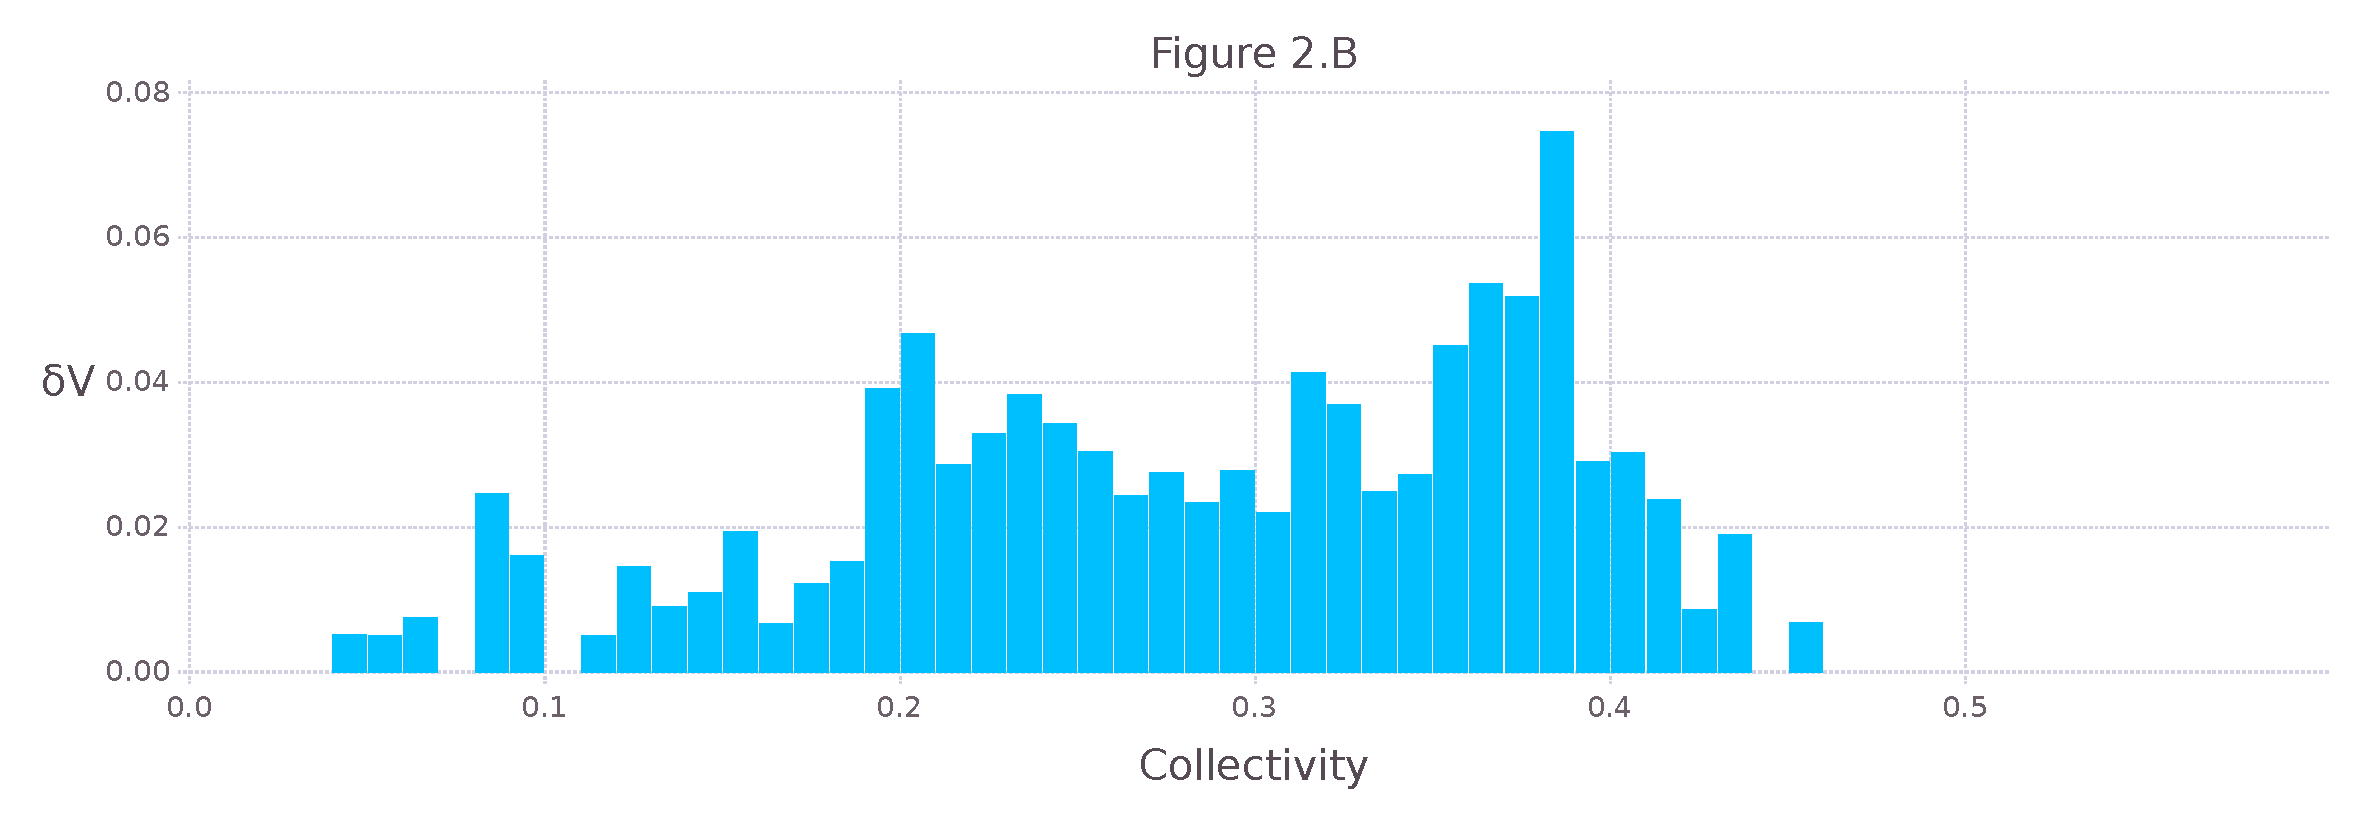
\includegraphics[scale=0.5]{1hvr_apo/2bfigure.pdf}
\caption{This is an inserted EPS graphic}
\label{fig5}
\end{center}
\end{figure}

\begin{figure}[ht]
\begin{center}
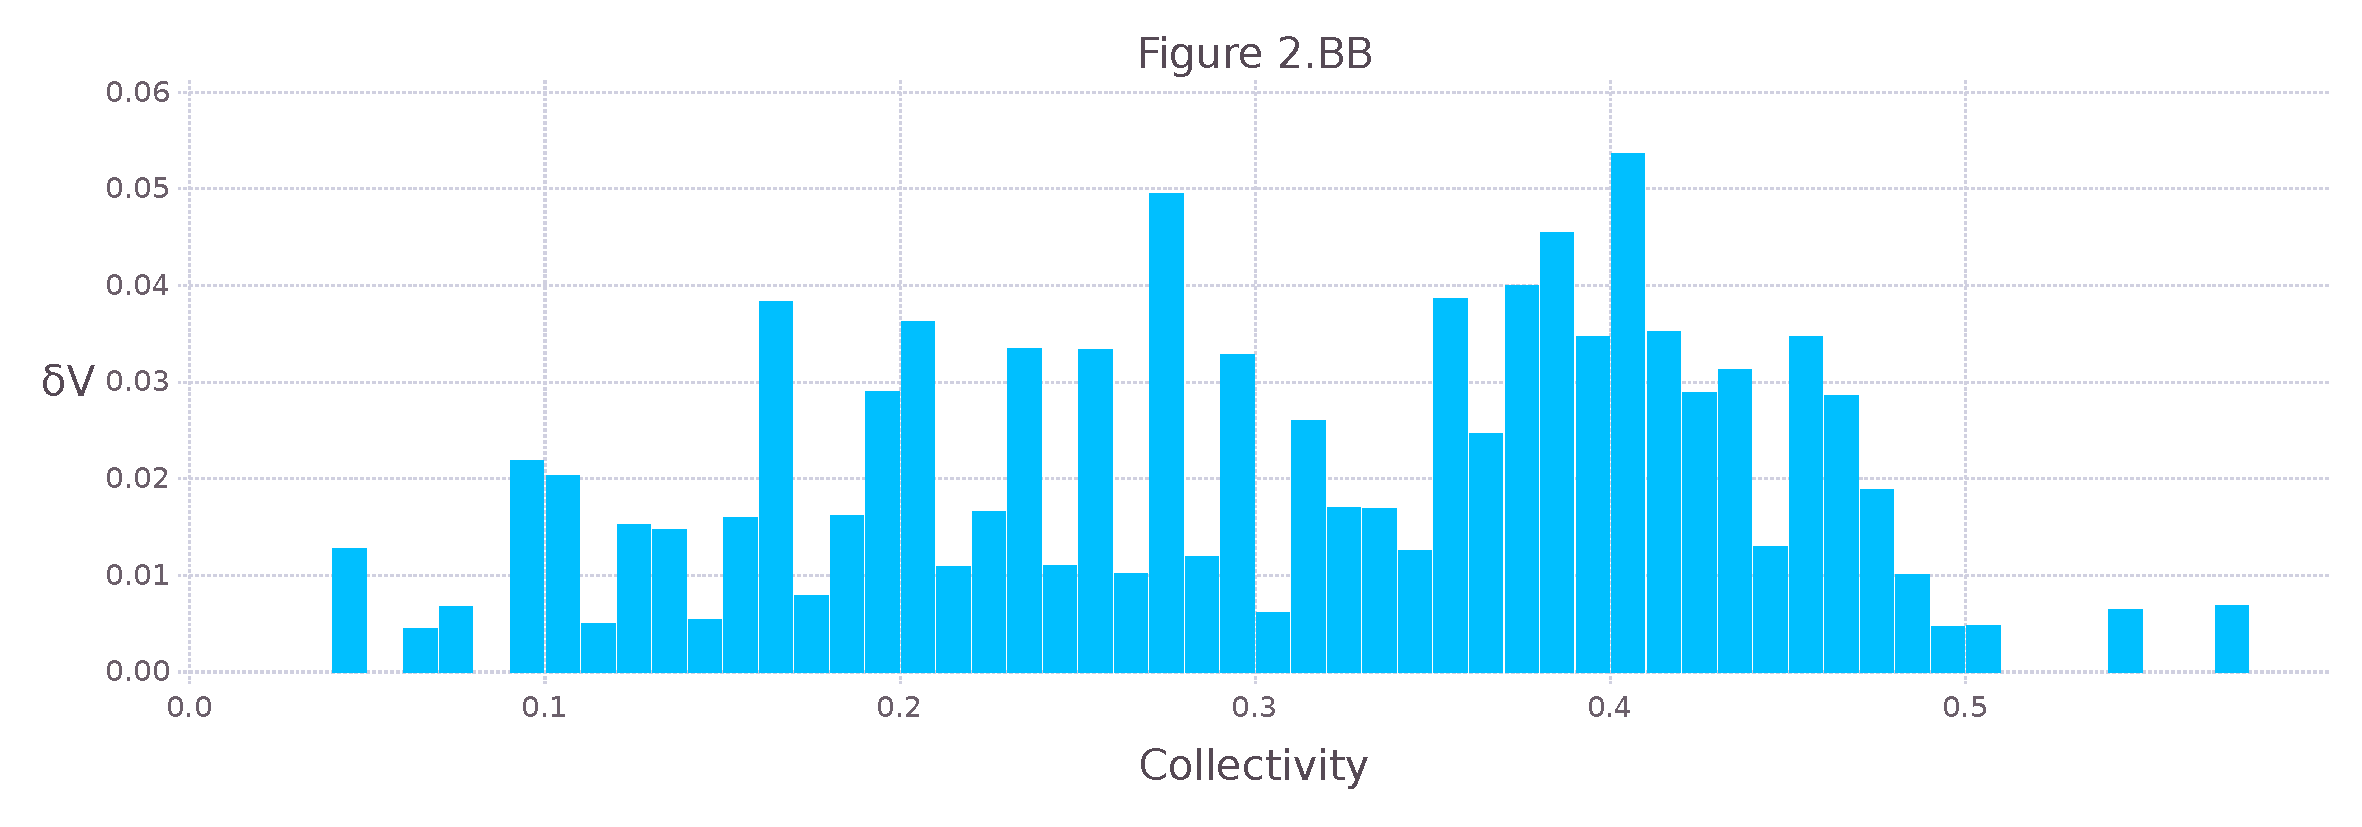
\includegraphics[scale=0.5]{1hvr_apo/2bbfigure.pdf}
\caption{This is an inserted EPS graphic}
\label{fig6}
\end{center}
\end{figure}


\clearpage
As in Fig.1, the analogous can be done with the \textbf{Participation Number}, as Fig.2 shows.

\begin{figure}[ht]
\begin{center}
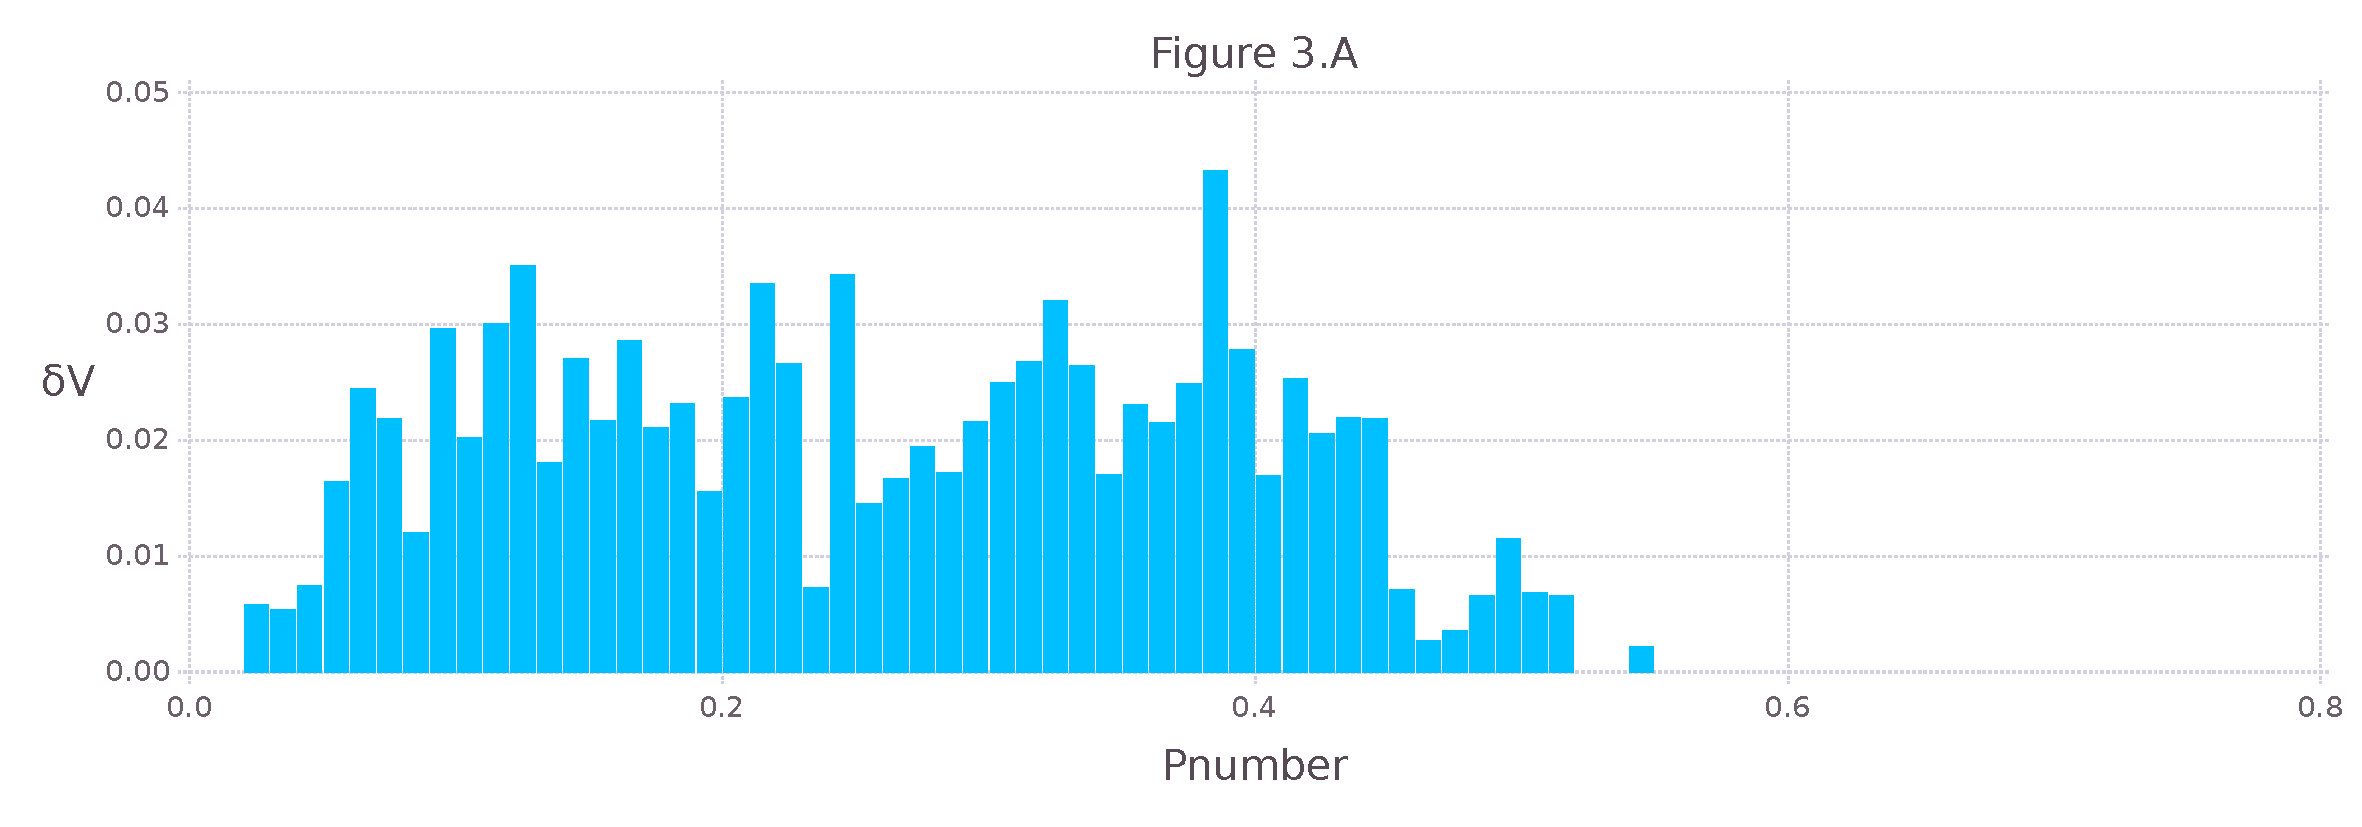
\includegraphics[scale=0.5]{1hvr_apo/3afigure.pdf}
\caption{This is an inserted EPS graphic}
\label{fig7}
\end{center}
\end{figure}

\begin{figure}[ht]
\begin{center}
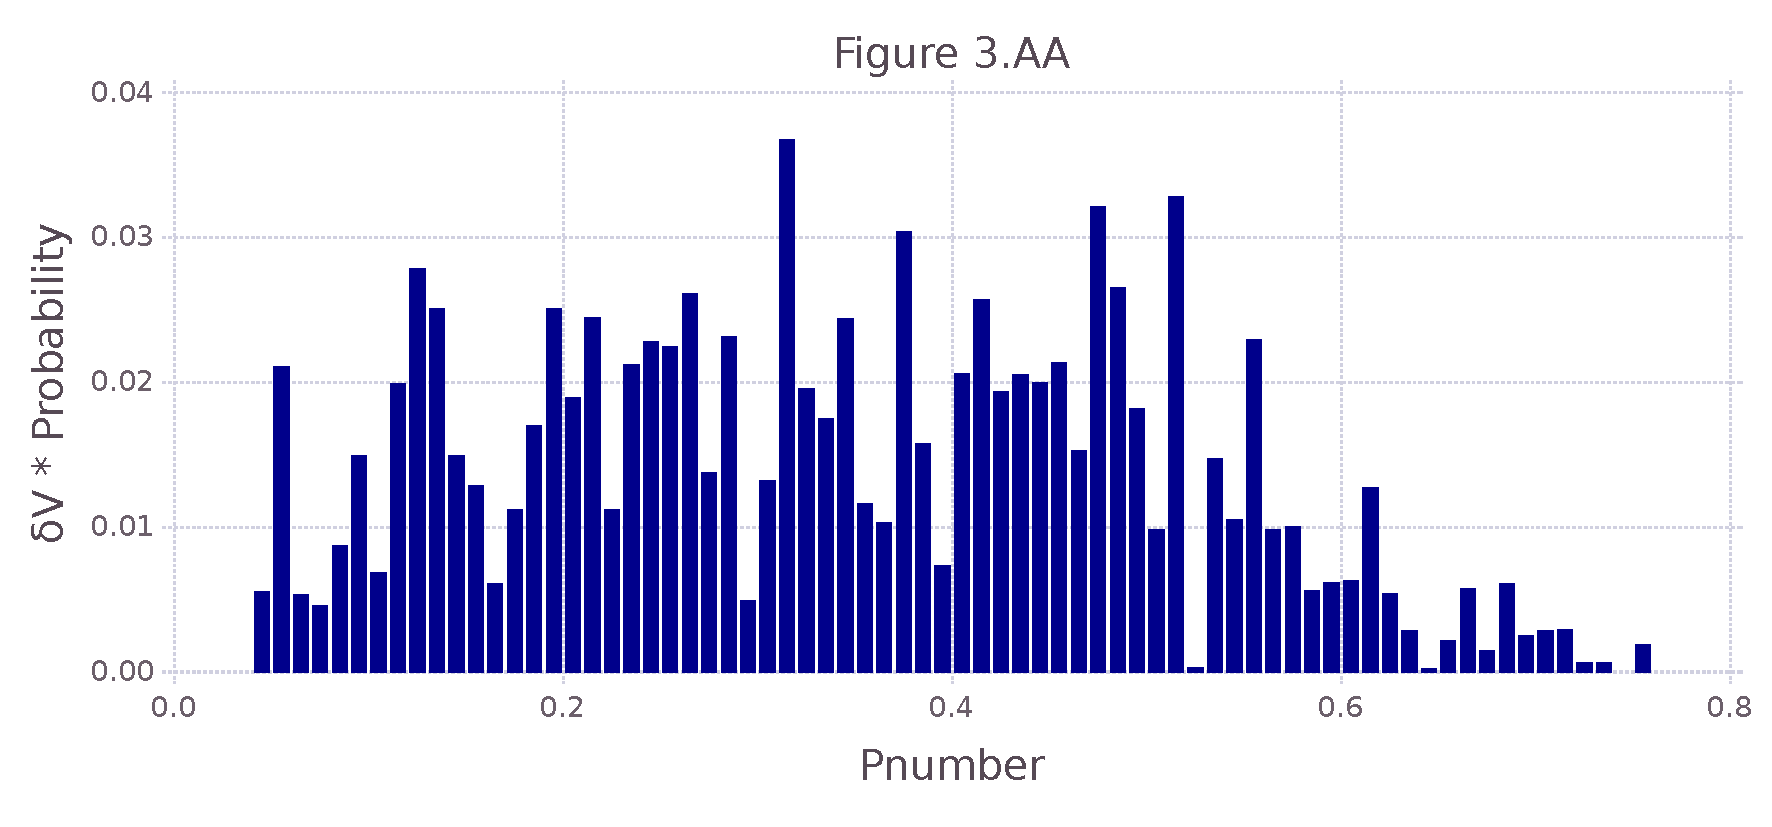
\includegraphics[scale=0.5]{1hvr_apo/3aafigure.pdf}
\caption{This is an inserted EPS graphic}
\label{fig8}
\end{center}
\end{figure}

\begin{figure}[ht]
\begin{center}
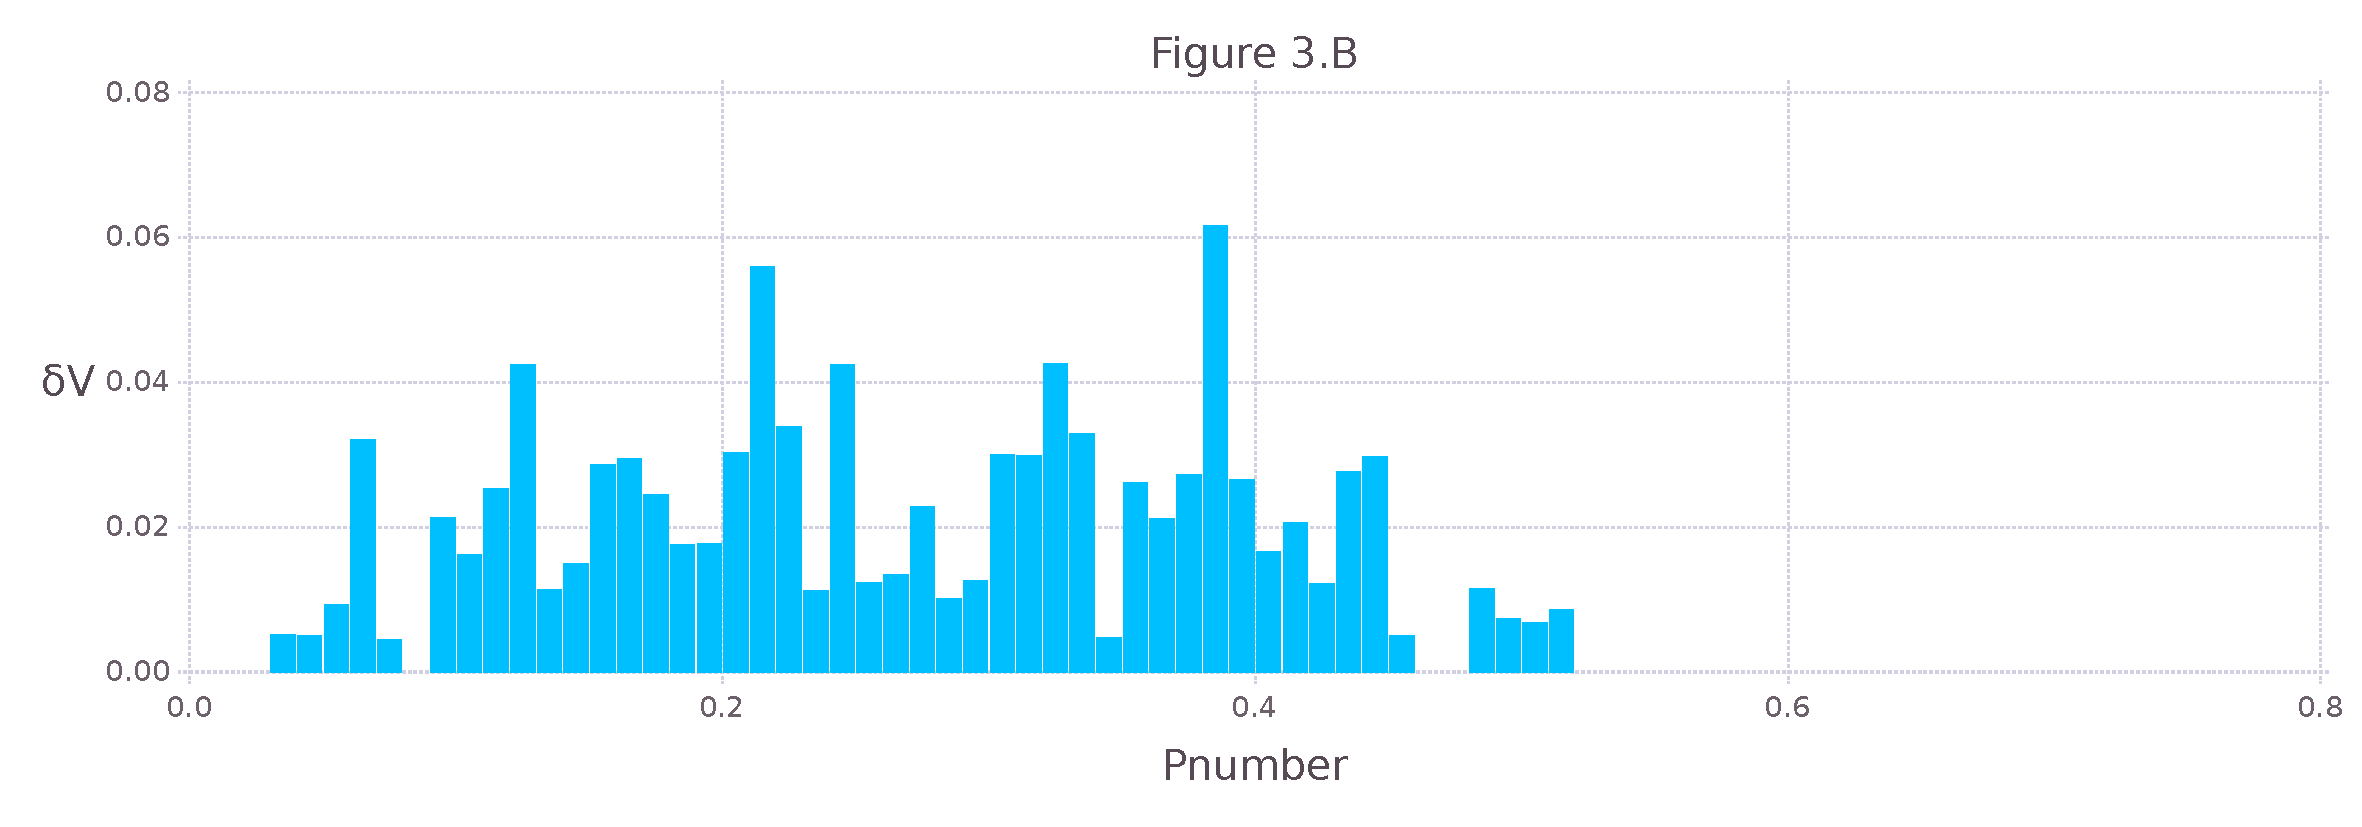
\includegraphics[scale=0.5]{1hvr_apo/3bfigure.pdf}
\caption{This is an inserted EPS graphic}
\label{fig10}
\end{center}
\end{figure}

\begin{figure}[ht]
\begin{center}
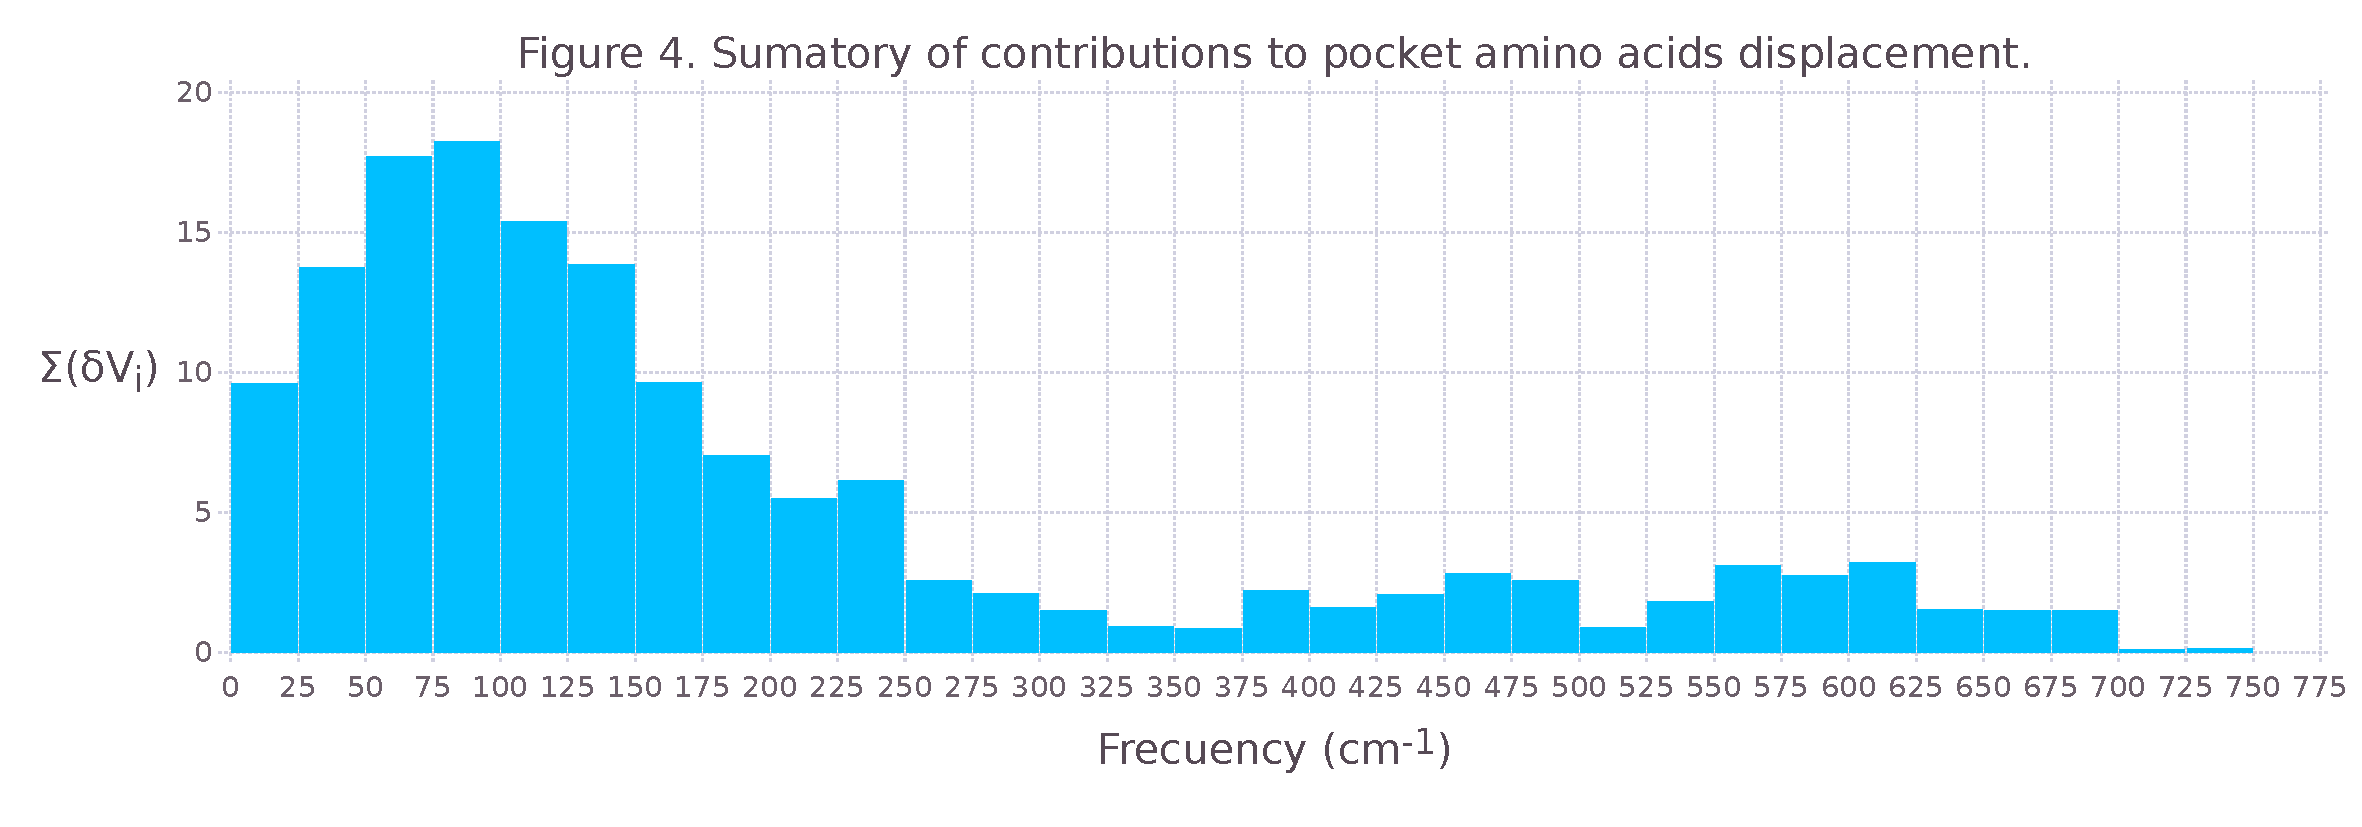
\includegraphics[scale=0.5]{1hvr_apo/3bbfigure.pdf}
\caption{This is an inserted EPS graphic}
\label{fig11}
\end{center}
\end{figure}

\begin{figure}[ht]
\begin{center}
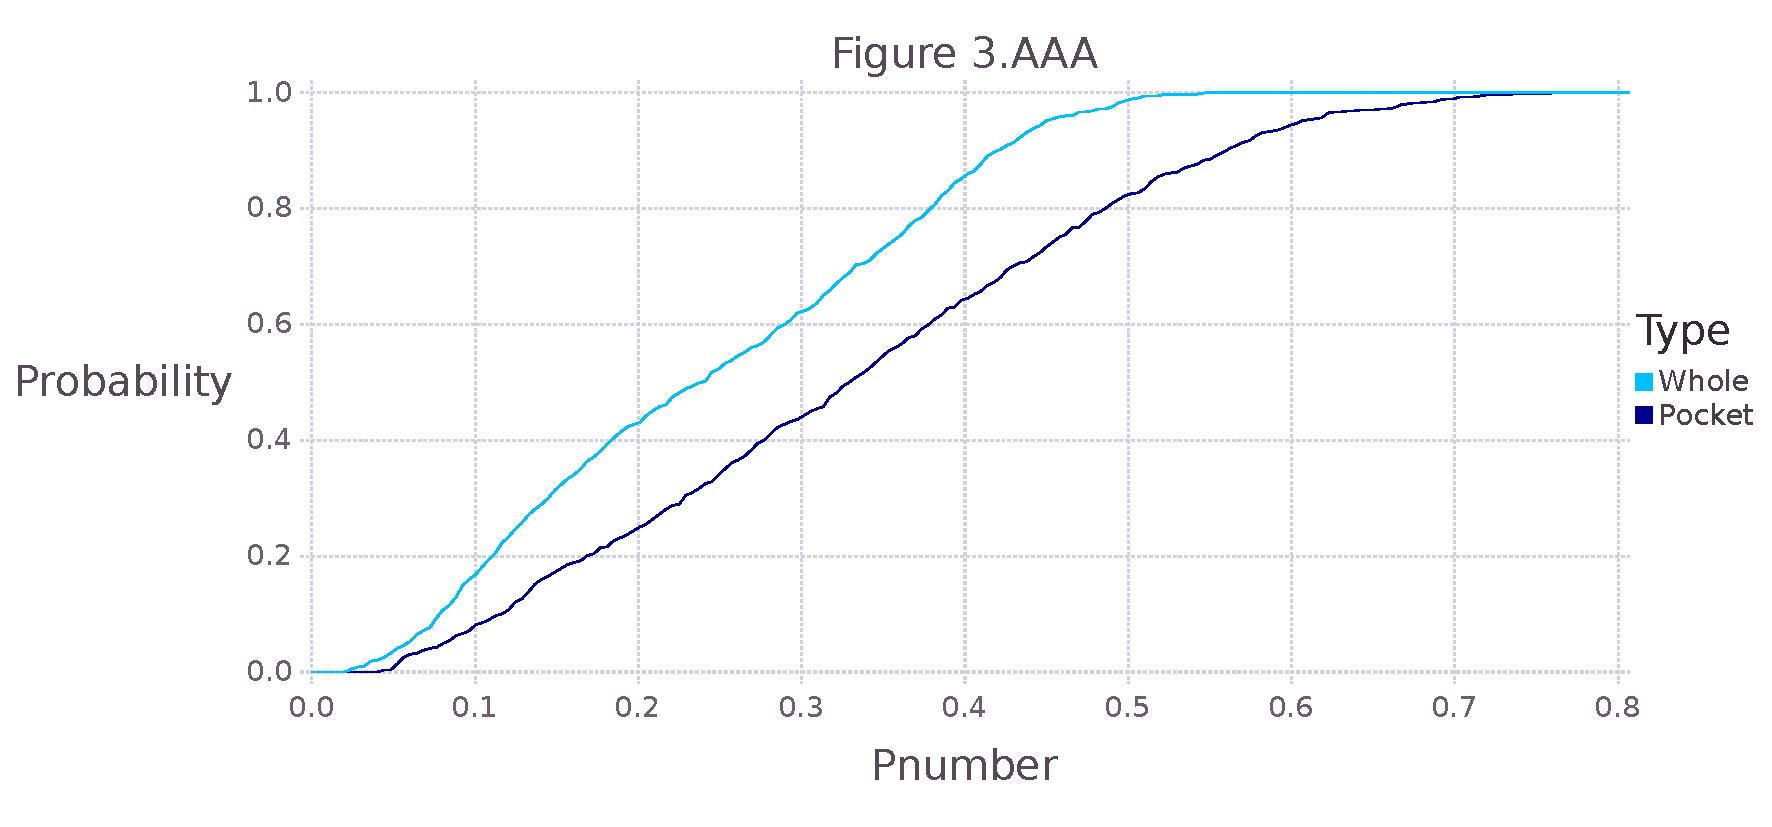
\includegraphics[scale=0.5]{1hvr_apo/3aaafigure.pdf}
\caption{This is an inserted EPS graphic}
\label{fig9}
\end{center}
\end{figure}

\begin{figure}[ht]
\begin{center}
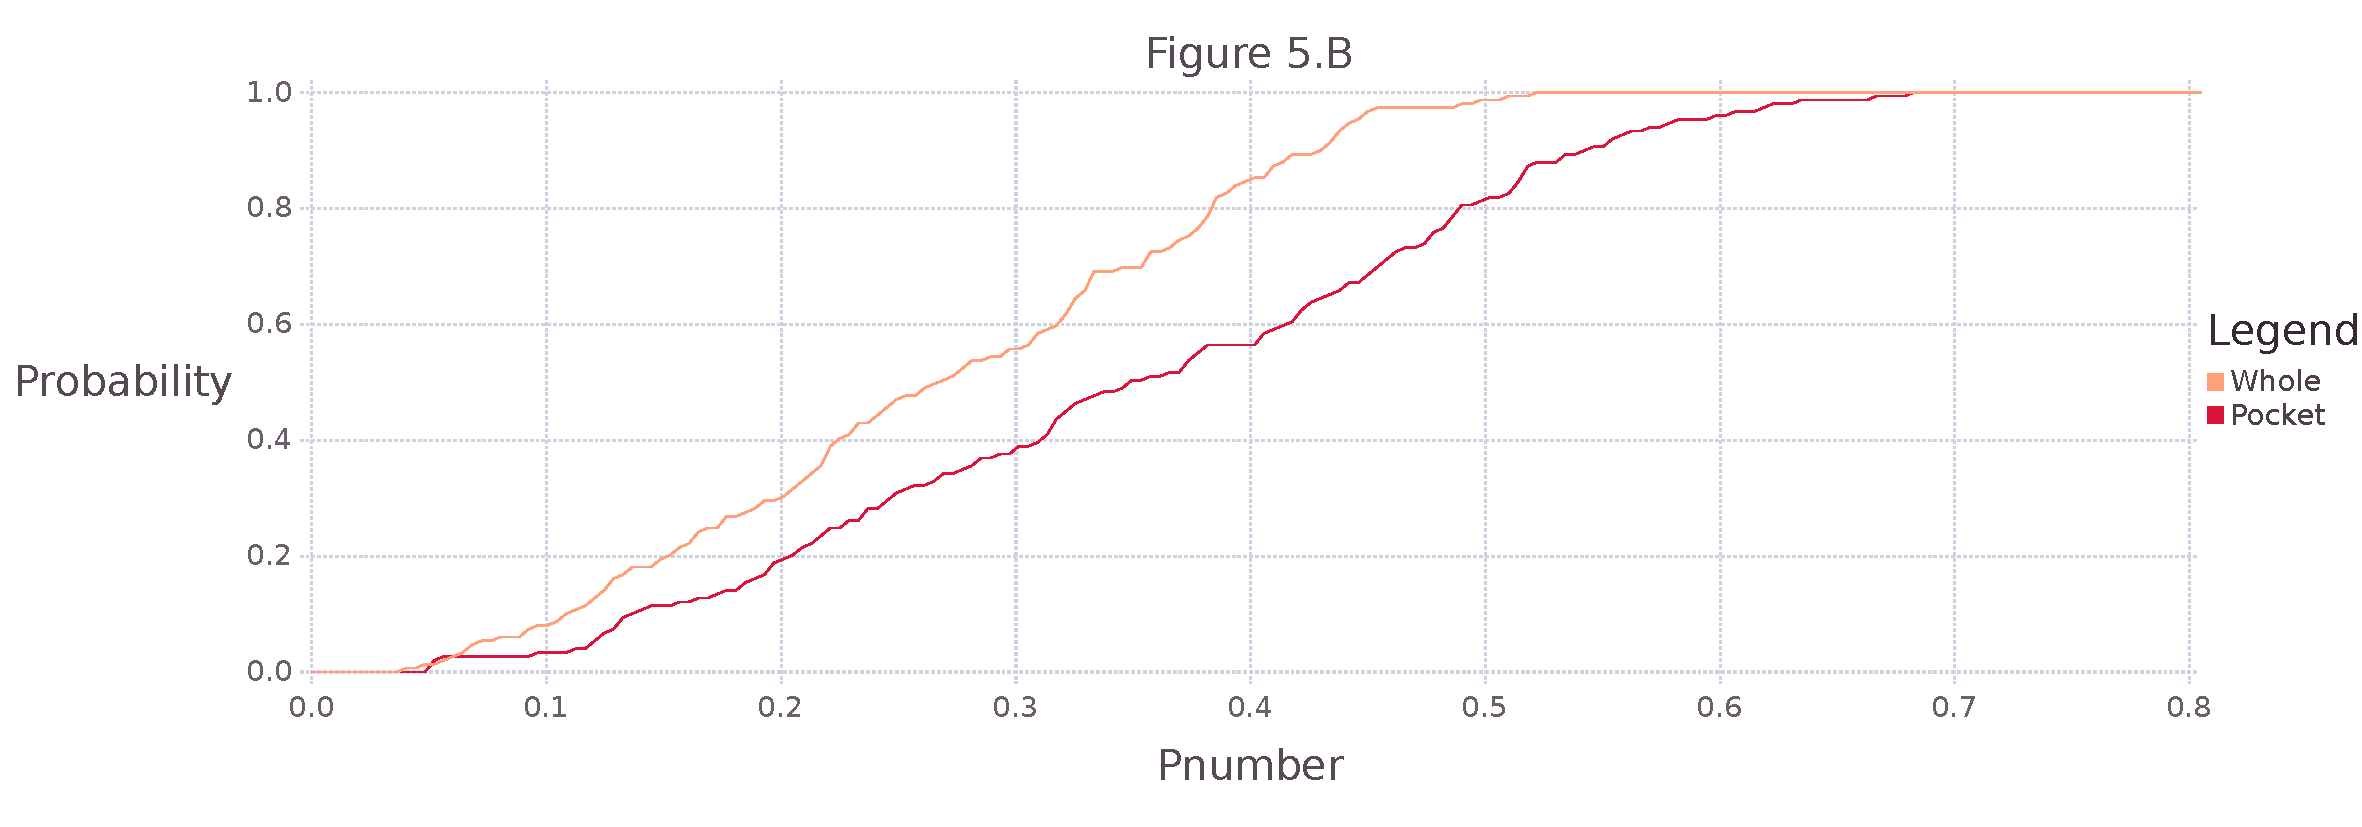
\includegraphics[scale=0.5]{1hvr_apo/3bbbfigure.pdf}
\caption{This is an inserted EPS graphic}
\label{fig12}
\end{center}
\end{figure}

\FloatBarrier


\textbf{VGV} can be translated into cartesian coordinates and the module of the \(X, Y, Z\) coordinates obtained.

\begin{figure}[ht]
\begin{center}
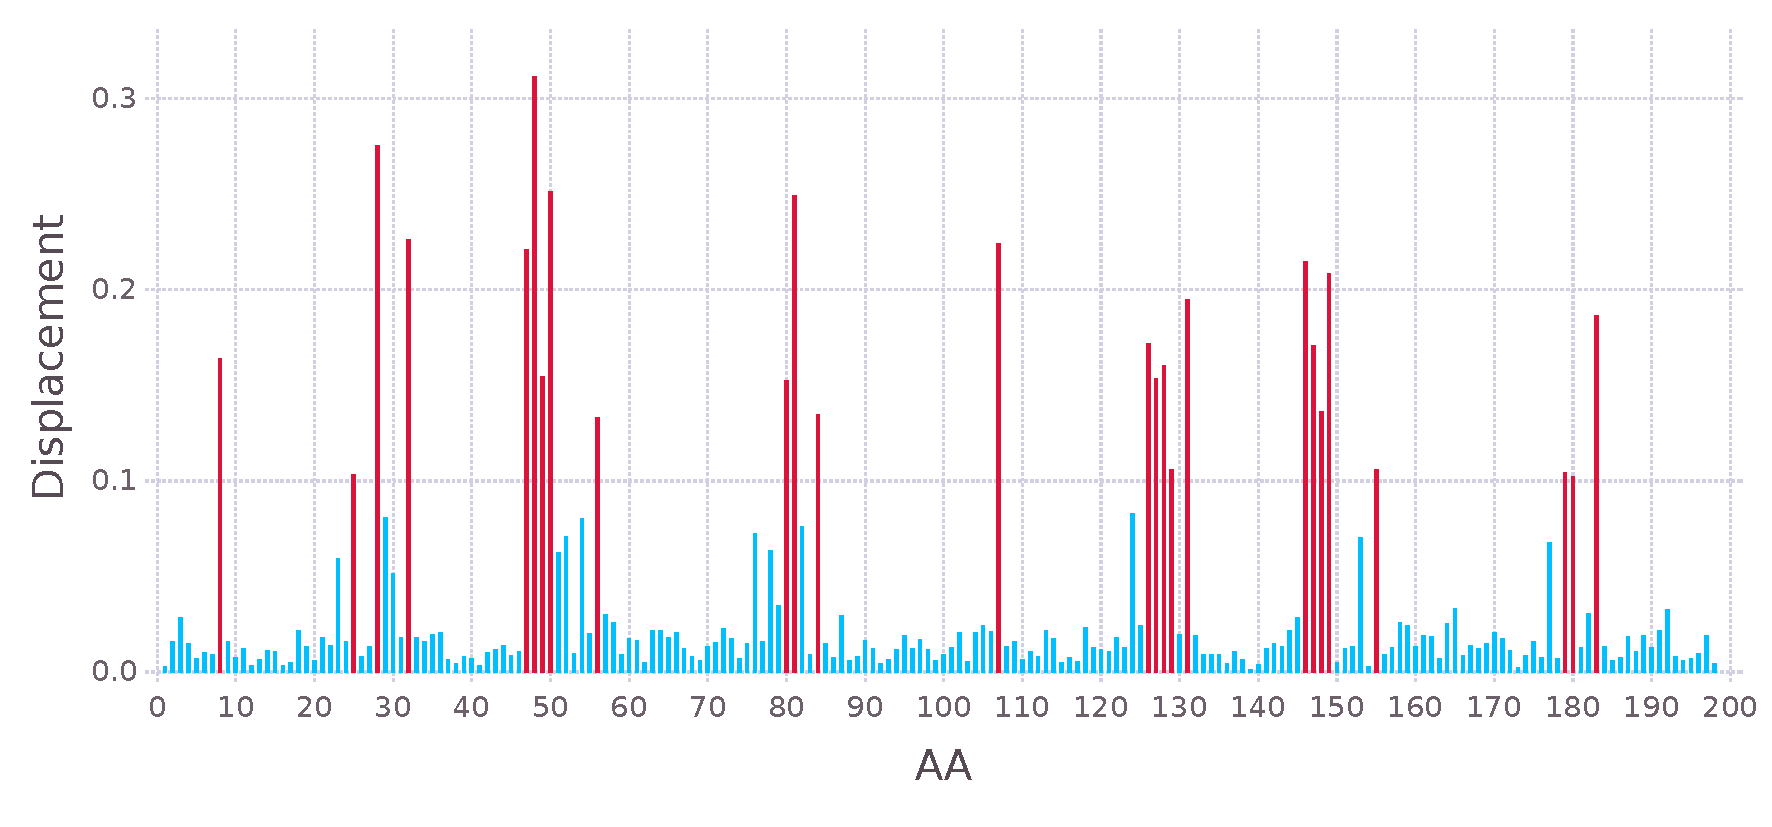
\includegraphics[scale=0.5]{1hvr_apo/5figure.pdf}
\caption{This is an inserted EPS graphic}
\label{fig13}
\end{center}
\end{figure}

\FloatBarrier
\newpage

\section{Discussion}

\newpage
\section{Supporting Information}
\subsection{Molecular Dynamics}
\label{Molecular Dynamics}
The 2 S-Hydroxycysteine amino acids in 1HVR were parametrized using the GAFF force field following AMBER developers recommendations. All molecules were simulated with leaprc.protein.ff14SB force field and solvated with TIP3P waters, forming a truncated octahedric box. Ions were added to neutralize each system.

All simulations were performed in the constant temperature and pressure (NTP) ensemble with T = 300K, P = 1bar, using the berendsen barostat and the Langevin thermostat with a \textbf{$\gamma$} collision frequency of 2 ps\textsuperscript{-1}

The simulation step was 2fs, water molecules and all bond lengths to hydrogen atoms were constrained using the SHAKE algorithm. Nonbonded interactions were cutoff at 10 \AA . Long-range electrostatic interactions were calculated using the Particle Mesh Ewald method.

Essential modes were extracted from the mass-weighted correlation matrix of the alpha carbon atoms. All \( {3*N-6} \) --- where \(N\) is the number of amino acids---, vectors were used for the calculations. 

%\section*{References}
% Either type in your references using
% \begin{thebibliography}{}
% \bibitem{}
% Text
% \end{thebibliography}
%
% OR
%
% Compile your BiBTeX database using our plos2015.bst
% style file and paste the contents of your .bbl file
% here.
% 
\newpage
\nolinenumbers
\begin{thebibliography}{10}

\bibitem{bib1}
Devaraju P, Gulati R, Antony PT, Mithun CB, Negi VS. Susceptibility to SLE in South Indian Tamils may be influenced by genetic selection pressure on TLR2 and TLR9 genes. Mol Immunol. 2014 Nov 22. pii: S0161-5890(14)00313-7. doi: 10.1016/j.molimm.2014.11.005

\end{thebibliography}
\end{document}

